\documentclass[man]{apa6}
\usepackage{lmodern}
\usepackage{amssymb,amsmath}
\usepackage{ifxetex,ifluatex}
\usepackage{fixltx2e} % provides \textsubscript
\ifnum 0\ifxetex 1\fi\ifluatex 1\fi=0 % if pdftex
  \usepackage[T1]{fontenc}
  \usepackage[utf8]{inputenc}
\else % if luatex or xelatex
  \ifxetex
    \usepackage{mathspec}
  \else
    \usepackage{fontspec}
  \fi
  \defaultfontfeatures{Ligatures=TeX,Scale=MatchLowercase}
\fi
% use upquote if available, for straight quotes in verbatim environments
\IfFileExists{upquote.sty}{\usepackage{upquote}}{}
% use microtype if available
\IfFileExists{microtype.sty}{%
\usepackage{microtype}
\UseMicrotypeSet[protrusion]{basicmath} % disable protrusion for tt fonts
}{}
\usepackage{hyperref}
\hypersetup{unicode=true,
            pdftitle={Power Analysis by Simulation using R, simglm, and Shiny},
            pdfauthor={Brandon LeBeau},
            pdfkeywords={power; simulation; R; simglm},
            pdfborder={0 0 0},
            breaklinks=true}
\urlstyle{same}  % don't use monospace font for urls
\usepackage{color}
\usepackage{fancyvrb}
\newcommand{\VerbBar}{|}
\newcommand{\VERB}{\Verb[commandchars=\\\{\}]}
\DefineVerbatimEnvironment{Highlighting}{Verbatim}{commandchars=\\\{\}}
% Add ',fontsize=\small' for more characters per line
\usepackage{framed}
\definecolor{shadecolor}{RGB}{248,248,248}
\newenvironment{Shaded}{\begin{snugshade}}{\end{snugshade}}
\newcommand{\AlertTok}[1]{\textcolor[rgb]{0.94,0.16,0.16}{#1}}
\newcommand{\AnnotationTok}[1]{\textcolor[rgb]{0.56,0.35,0.01}{\textbf{\textit{#1}}}}
\newcommand{\AttributeTok}[1]{\textcolor[rgb]{0.77,0.63,0.00}{#1}}
\newcommand{\BaseNTok}[1]{\textcolor[rgb]{0.00,0.00,0.81}{#1}}
\newcommand{\BuiltInTok}[1]{#1}
\newcommand{\CharTok}[1]{\textcolor[rgb]{0.31,0.60,0.02}{#1}}
\newcommand{\CommentTok}[1]{\textcolor[rgb]{0.56,0.35,0.01}{\textit{#1}}}
\newcommand{\CommentVarTok}[1]{\textcolor[rgb]{0.56,0.35,0.01}{\textbf{\textit{#1}}}}
\newcommand{\ConstantTok}[1]{\textcolor[rgb]{0.00,0.00,0.00}{#1}}
\newcommand{\ControlFlowTok}[1]{\textcolor[rgb]{0.13,0.29,0.53}{\textbf{#1}}}
\newcommand{\DataTypeTok}[1]{\textcolor[rgb]{0.13,0.29,0.53}{#1}}
\newcommand{\DecValTok}[1]{\textcolor[rgb]{0.00,0.00,0.81}{#1}}
\newcommand{\DocumentationTok}[1]{\textcolor[rgb]{0.56,0.35,0.01}{\textbf{\textit{#1}}}}
\newcommand{\ErrorTok}[1]{\textcolor[rgb]{0.64,0.00,0.00}{\textbf{#1}}}
\newcommand{\ExtensionTok}[1]{#1}
\newcommand{\FloatTok}[1]{\textcolor[rgb]{0.00,0.00,0.81}{#1}}
\newcommand{\FunctionTok}[1]{\textcolor[rgb]{0.00,0.00,0.00}{#1}}
\newcommand{\ImportTok}[1]{#1}
\newcommand{\InformationTok}[1]{\textcolor[rgb]{0.56,0.35,0.01}{\textbf{\textit{#1}}}}
\newcommand{\KeywordTok}[1]{\textcolor[rgb]{0.13,0.29,0.53}{\textbf{#1}}}
\newcommand{\NormalTok}[1]{#1}
\newcommand{\OperatorTok}[1]{\textcolor[rgb]{0.81,0.36,0.00}{\textbf{#1}}}
\newcommand{\OtherTok}[1]{\textcolor[rgb]{0.56,0.35,0.01}{#1}}
\newcommand{\PreprocessorTok}[1]{\textcolor[rgb]{0.56,0.35,0.01}{\textit{#1}}}
\newcommand{\RegionMarkerTok}[1]{#1}
\newcommand{\SpecialCharTok}[1]{\textcolor[rgb]{0.00,0.00,0.00}{#1}}
\newcommand{\SpecialStringTok}[1]{\textcolor[rgb]{0.31,0.60,0.02}{#1}}
\newcommand{\StringTok}[1]{\textcolor[rgb]{0.31,0.60,0.02}{#1}}
\newcommand{\VariableTok}[1]{\textcolor[rgb]{0.00,0.00,0.00}{#1}}
\newcommand{\VerbatimStringTok}[1]{\textcolor[rgb]{0.31,0.60,0.02}{#1}}
\newcommand{\WarningTok}[1]{\textcolor[rgb]{0.56,0.35,0.01}{\textbf{\textit{#1}}}}
\usepackage{graphicx,grffile}
\makeatletter
\def\maxwidth{\ifdim\Gin@nat@width>\linewidth\linewidth\else\Gin@nat@width\fi}
\def\maxheight{\ifdim\Gin@nat@height>\textheight\textheight\else\Gin@nat@height\fi}
\makeatother
% Scale images if necessary, so that they will not overflow the page
% margins by default, and it is still possible to overwrite the defaults
% using explicit options in \includegraphics[width, height, ...]{}
\setkeys{Gin}{width=\maxwidth,height=\maxheight,keepaspectratio}
\IfFileExists{parskip.sty}{%
\usepackage{parskip}
}{% else
\setlength{\parindent}{0pt}
\setlength{\parskip}{6pt plus 2pt minus 1pt}
}
\setlength{\emergencystretch}{3em}  % prevent overfull lines
\providecommand{\tightlist}{%
  \setlength{\itemsep}{0pt}\setlength{\parskip}{0pt}}
\setcounter{secnumdepth}{0}
% Redefines (sub)paragraphs to behave more like sections
\ifx\paragraph\undefined\else
\let\oldparagraph\paragraph
\renewcommand{\paragraph}[1]{\oldparagraph{#1}\mbox{}}
\fi
\ifx\subparagraph\undefined\else
\let\oldsubparagraph\subparagraph
\renewcommand{\subparagraph}[1]{\oldsubparagraph{#1}\mbox{}}
\fi

%%% Use protect on footnotes to avoid problems with footnotes in titles
\let\rmarkdownfootnote\footnote%
\def\footnote{\protect\rmarkdownfootnote}


  \title{Power Analysis by Simulation using R, simglm, and Shiny}
    \author{Brandon LeBeau\textsuperscript{1}}
    \date{}
  
\shorttitle{Power by Simulation}
\affiliation{
\vspace{0.5cm}
\textsuperscript{1} University of Iowa}
\keywords{power; simulation; R; simglm\newline\indent Word count: X}
\usepackage{csquotes}
\usepackage{upgreek}
\captionsetup{font=singlespacing,justification=justified}

\usepackage{longtable}
\usepackage{lscape}
\usepackage{multirow}
\usepackage{tabularx}
\usepackage[flushleft]{threeparttable}
\usepackage{threeparttablex}

\newenvironment{lltable}{\begin{landscape}\begin{center}\begin{ThreePartTable}}{\end{ThreePartTable}\end{center}\end{landscape}}

\makeatletter
\newcommand\LastLTentrywidth{1em}
\newlength\longtablewidth
\setlength{\longtablewidth}{1in}
\newcommand{\getlongtablewidth}{\begingroup \ifcsname LT@\roman{LT@tables}\endcsname \global\longtablewidth=0pt \renewcommand{\LT@entry}[2]{\global\advance\longtablewidth by ##2\relax\gdef\LastLTentrywidth{##2}}\@nameuse{LT@\roman{LT@tables}} \fi \endgroup}


\DeclareDelayedFloatFlavor{ThreePartTable}{table}
\DeclareDelayedFloatFlavor{lltable}{table}
\DeclareDelayedFloatFlavor*{longtable}{table}
\makeatletter
\renewcommand{\efloat@iwrite}[1]{\immediate\expandafter\protected@write\csname efloat@post#1\endcsname{}}
\makeatother

\authornote{Department of Psychological and Quantitative Foundations

Correspondence concerning this article should be addressed to Brandon LeBeau, Postal address. E-mail: \href{mailto:brandon-lebeau@uiowa.edu}{\nolinkurl{brandon-lebeau@uiowa.edu}}}

\abstract{

}

\begin{document}
\maketitle

Statistical power is the probability that a statistical analysis is able to detect a non-zero population effect for a binary hypothesis test. In probability terms, statistical power reflects the probability of correctly rejecting the null hypothesis when it is false in the population or mathematically as: \(power = P(reject \; H_{0} \; | \; H_{1} \; is \; true)\). The inverse of power is the probability of making a type II error or the false negative rate.

Power analyses can take on two forms, a priori power analyses occur prior to collecting data and post hoc power analyses occur after data analysis. Post hoc power analyses are controversial, can be misleading given the analysis has already been done, and can give inaccurate results when calculating power using sample data. Therefore, this paper will focus on a priori power analyses, however the process described in this paper could be applied to post hoc power analyses.

\hypertarget{factors-affecting-power}{%
\subsection{Factors affecting power}\label{factors-affecting-power}}

There are numerous known factors that can impact power in a given analysis. The most well known include sample size, the alpha rate or false positive rate, and the magnitude of the effect size. Other factors such as statistical design, statistical analysis, missing data, or whether statistical assumptions have been met.

\hypertarget{traditional-procedures-for-power}{%
\section{Traditional procedures for power}\label{traditional-procedures-for-power}}

Power is often evaluated using closed form solutions that assume statistical assumptions hold. For example, residuals for many statistical analyses are assumed to follow a normal distribution.

Statistical software has been developed to estimate power when these statistical assumptions have been made such as \href{http://www.gpower.hhu.de/}{G*Power}, \href{https://www.causalevaluation.org/power-analysis.html}{PowerUp!}, or \href{http://hlmsoft.net/od/}{Optimal Design}. There are also packages in statistical software programs such as \href{https://cran.r-project.org/package=pwr}{pwr}, \href{https://cran.r-project.org/package=WebPower}{WebPower}, or \href{https://cran.r-project.org/package=STAT}{stats} in R or \href{http://www.statsmodels.org/}{statsmodels} in Python that estimate power for relatively simple statistical analyses such as t-tests, analysis of variance (ANOVA), linear regression, correlation, or general linear models. G*Power implements power for similar analyses as those found in traditional statistcal software implementations, but offers a graphical user interface (GUI) that may aid users in the power estimation. Finally, the specialized software, PowerUp! and Optimal Design are commonly used to estimate power for randomized control trials and when there are nesting effects that are common in educational or pscyhological research.

Power can be estimated to explore what the probability is given a specific effect size. The minimum detectable effect size given specific sample sizes can also be estimated for power analyses. The latter is often estimated when writing grant applications where the minimum detectable effect size is estimated for specified power levels. Regardless of the framework, it needs to be articulated whether the effect size is of substantive interest and large enough to have a meaningful effect in the population.

\hypertarget{power-by-simulation}{%
\section{Power by Simulation}\label{power-by-simulation}}

Power by simulation differs from the traditional approaches in that it is able to be flexible to evaluate the impact on power when statistical assumptions are not met or under different missing data mechanisms which may better reflect realistic data collection conditions.

The following are genearl steps that are taken in a power by simulation example.

\begin{enumerate}
\def\labelenumi{\arabic{enumi}.}
\tightlist
\item
  Assume population parameters, including

  \begin{itemize}
  \tightlist
  \item
    population effect size(s) of interest.
  \item
    distribution of variable(s) and residuals.
  \item
    variance of variable(s) and residuals.
  \end{itemize}
\item
  Simulate data based on a statistical model.
\item
  Fit a statistical model to the simulated data.
\item
  Replicate steps 1 - 3 many times.
\item
  Calculate the proportion of statistical tests that appropriate reject the null hypothesis.
\end{enumerate}

In the power by simulation framework, data are simulated based on assumed values for the population, for example the population mean difference between two groups. Given that these values are true, data are simulated many times, replicated, and a statistical model is fitted to the simulated data. To estimate power in this framework, the number of statistical tests that properly reject the null hypothesis compared to the number of replications

\hypertarget{benefits-of-power-by-simulation}{%
\subsection{Benefits of Power by Simulation}\label{benefits-of-power-by-simulation}}

Power by simulation can be used for any statistical design or statistical analysis. The limiting factor is the ability of the researcher to use statistical software to follow the steps outlined above. Power by simulation can allow researchers to relax statistical assumptions that may have an impact on statistical power and more readily mirror real data conditions. If statistical assumptions do not hold in the population, the power analysis that makes these assumptions will commonly overestimate power. This can have important considerations and implications for researchers, funders, or other relavent stakeholders that are invested in the research idea.

Furthermore, as power by simulation is not limited by the software and the steps for employing a power by simulation analysis are the same regardless of the statistical design or analysis, once the process of simluation by power are well understood, the only major change across different statistical designs and analysis are the generating and fitted models. In some cases, getting estimates of population effects may be more challenging as the model complexity increases, but this can be a limiting factor of traditional power analyses as well.

\hypertarget{two-sample-t-test-example}{%
\section{Two-Sample t-test Example}\label{two-sample-t-test-example}}

Power for a two-sample design using the t-test can be done with the following code for a single effect size, standardized mean difference of 0.15. This example generates power for sample sizes ranging from 4 up to 1000 increasing by intervals of 2. This will generate power values for 499 sample sizes.

\begin{Shaded}
\begin{Highlighting}[]
\KeywordTok{library}\NormalTok{(tidyverse)}
\KeywordTok{library}\NormalTok{(simglm)}
\KeywordTok{library}\NormalTok{(future.apply)}
\KeywordTok{library}\NormalTok{(lme4)}
\end{Highlighting}
\end{Shaded}

\begin{Shaded}
\begin{Highlighting}[]
\NormalTok{n <-}\StringTok{ }\KeywordTok{seq}\NormalTok{(}\DecValTok{4}\NormalTok{, }\DecValTok{1000}\NormalTok{, }\DecValTok{2}\NormalTok{)}
\NormalTok{power <-}\StringTok{ }\KeywordTok{sapply}\NormalTok{(}\KeywordTok{seq_along}\NormalTok{(n), }\ControlFlowTok{function}\NormalTok{(i) }
  \KeywordTok{power.t.test}\NormalTok{(}\DataTypeTok{n =}\NormalTok{ n[i], }\DataTypeTok{delta =} \FloatTok{.15}\NormalTok{, }\DataTypeTok{sd =} \DecValTok{1}\NormalTok{, }\DataTypeTok{type =} \StringTok{'two.sample'}\NormalTok{)}\OperatorTok{$}\NormalTok{power)}
\end{Highlighting}
\end{Shaded}

The power for the first iteration can be extracted directly using \texttt{power{[}1{]}} 0.04, but generally showing a figure would be more interesting.

\begin{Shaded}
\begin{Highlighting}[]
\NormalTok{power_df <-}\StringTok{ }\KeywordTok{data.frame}\NormalTok{(}
  \DataTypeTok{n =}\NormalTok{ n,}
  \DataTypeTok{power =}\NormalTok{ power}
\NormalTok{)}

\KeywordTok{ggplot}\NormalTok{(power_df, }\KeywordTok{aes}\NormalTok{(}\DataTypeTok{x =}\NormalTok{ n, }\DataTypeTok{y =}\NormalTok{ power)) }\OperatorTok{+}\StringTok{ }
\StringTok{  }\KeywordTok{geom_line}\NormalTok{(}\DataTypeTok{size =} \DecValTok{2}\NormalTok{) }\OperatorTok{+}\StringTok{ }
\StringTok{  }\KeywordTok{geom_hline}\NormalTok{(}\DataTypeTok{yintercept =} \FloatTok{0.8}\NormalTok{, }\DataTypeTok{linetype =} \DecValTok{2}\NormalTok{, }\DataTypeTok{color =} \StringTok{'gray30'}\NormalTok{) }\OperatorTok{+}\StringTok{ }
\StringTok{  }\KeywordTok{geom_vline}\NormalTok{(}\DataTypeTok{xintercept =} \DecValTok{700}\NormalTok{, }\DataTypeTok{linetype =} \DecValTok{2}\NormalTok{, }\DataTypeTok{color =} \StringTok{'gray30'}\NormalTok{) }\OperatorTok{+}
\StringTok{  }\KeywordTok{scale_x_continuous}\NormalTok{(}\StringTok{"Sample Size"}\NormalTok{, }\DataTypeTok{breaks =} \KeywordTok{seq}\NormalTok{(}\DecValTok{0}\NormalTok{, }\DecValTok{1000}\NormalTok{, }\DecValTok{200}\NormalTok{)) }\OperatorTok{+}\StringTok{ }
\StringTok{  }\KeywordTok{scale_y_continuous}\NormalTok{(}\StringTok{"Power"}\NormalTok{, }\DataTypeTok{breaks =} \KeywordTok{seq}\NormalTok{(}\DecValTok{0}\NormalTok{, }\DecValTok{1}\NormalTok{, }\FloatTok{.2}\NormalTok{)) }\OperatorTok{+}
\StringTok{  }\KeywordTok{theme_bw}\NormalTok{(}\DataTypeTok{base_size =} \DecValTok{14}\NormalTok{)}
\end{Highlighting}
\end{Shaded}

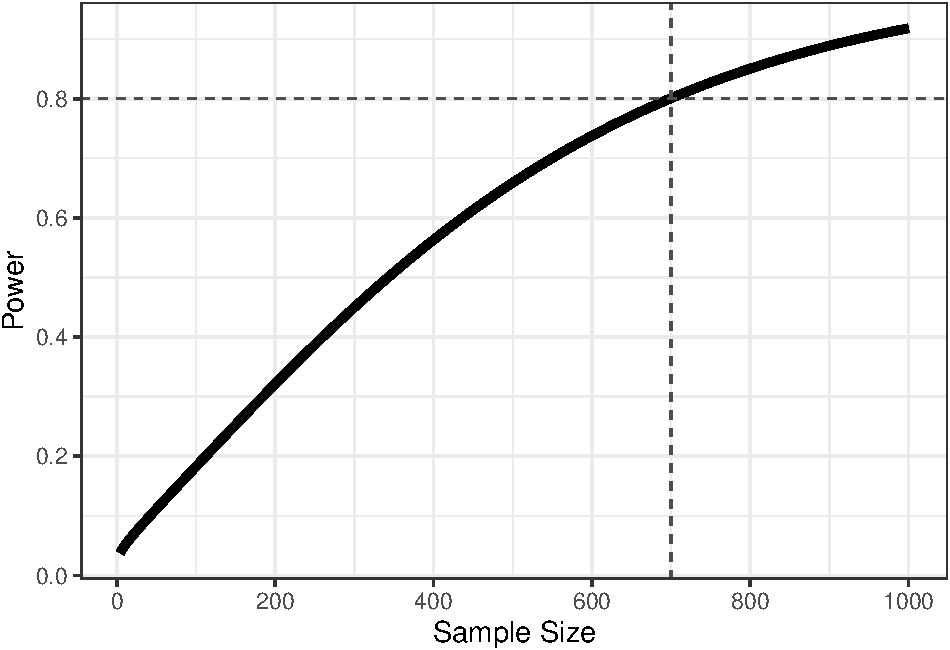
\includegraphics{power_simulation_files/figure-latex/power-figure-1.pdf}

\hypertarget{power-curves}{%
\subsection{Power Curves}\label{power-curves}}

It is common for the effect size of interest to not be completely certain a priori when many power analyses are conducted. In these cases, a form of sensitivity analysis or descriptive power analyses are often conducted that vary the effect size as well.

A similar structure can be done to add the power curves for different effect sizes; the primary differences being the addition of different effect sizes in addition to the different sample size conditions.

\begin{Shaded}
\begin{Highlighting}[]
\NormalTok{effect_sizes <-}\StringTok{ }\KeywordTok{c}\NormalTok{(.}\DecValTok{10}\NormalTok{, }\FloatTok{.15}\NormalTok{, }\FloatTok{.25}\NormalTok{)}
\NormalTok{conditions <-}\StringTok{ }\KeywordTok{expand.grid}\NormalTok{(}\DataTypeTok{n =}\NormalTok{ n, }\DataTypeTok{effect_sizes =}\NormalTok{ effect_sizes)}
\KeywordTok{head}\NormalTok{(conditions)}
\end{Highlighting}
\end{Shaded}

\begin{verbatim}
##    n effect_sizes
## 1  4          0.1
## 2  6          0.1
## 3  8          0.1
## 4 10          0.1
## 5 12          0.1
## 6 14          0.1
\end{verbatim}

\begin{Shaded}
\begin{Highlighting}[]
\NormalTok{power_curve <-}\StringTok{ }\KeywordTok{sapply}\NormalTok{(}\KeywordTok{seq_len}\NormalTok{(}\KeywordTok{nrow}\NormalTok{(conditions)), }\ControlFlowTok{function}\NormalTok{(i) }
  \KeywordTok{power.t.test}\NormalTok{(}\DataTypeTok{n =}\NormalTok{ conditions[i, }\StringTok{'n'}\NormalTok{], }
               \DataTypeTok{delta =}\NormalTok{ conditions[i, }\StringTok{'effect_sizes'}\NormalTok{], }
               \DataTypeTok{sd =} \DecValTok{1}\NormalTok{, }\DataTypeTok{type =} \StringTok{'two.sample'}\NormalTok{)}\OperatorTok{$}\NormalTok{power)}
\end{Highlighting}
\end{Shaded}

These can then be visualized after converting to a data frame and combining with the original conditions object.

\begin{Shaded}
\begin{Highlighting}[]
\NormalTok{power_curve_df <-}\StringTok{ }\KeywordTok{bind_cols}\NormalTok{(}
\NormalTok{  conditions, }
  \DataTypeTok{power =}\NormalTok{ power_curve}
\NormalTok{)}

\KeywordTok{ggplot}\NormalTok{(power_curve_df, }\KeywordTok{aes}\NormalTok{(}\DataTypeTok{x =}\NormalTok{ n, }\DataTypeTok{y =}\NormalTok{ power)) }\OperatorTok{+}\StringTok{ }
\StringTok{  }\KeywordTok{geom_line}\NormalTok{(}\KeywordTok{aes}\NormalTok{(}\DataTypeTok{color =} \KeywordTok{factor}\NormalTok{(effect_sizes)), }\DataTypeTok{size =} \DecValTok{2}\NormalTok{) }\OperatorTok{+}\StringTok{ }
\StringTok{  }\KeywordTok{geom_hline}\NormalTok{(}\DataTypeTok{yintercept =} \FloatTok{0.8}\NormalTok{, }\DataTypeTok{linetype =} \DecValTok{2}\NormalTok{, }\DataTypeTok{color =} \StringTok{'gray30'}\NormalTok{) }\OperatorTok{+}\StringTok{ }
\StringTok{  }\CommentTok{#geom_vline(xintercept = 700, linetype = 2, color = 'gray30') +}
\StringTok{  }\KeywordTok{scale_x_continuous}\NormalTok{(}\StringTok{"Sample Size"}\NormalTok{, }\DataTypeTok{breaks =} \KeywordTok{seq}\NormalTok{(}\DecValTok{0}\NormalTok{, }\DecValTok{1000}\NormalTok{, }\DecValTok{200}\NormalTok{)) }\OperatorTok{+}\StringTok{ }
\StringTok{  }\KeywordTok{scale_y_continuous}\NormalTok{(}\StringTok{"Power"}\NormalTok{, }\DataTypeTok{breaks =} \KeywordTok{seq}\NormalTok{(}\DecValTok{0}\NormalTok{, }\DecValTok{1}\NormalTok{, }\FloatTok{.2}\NormalTok{)) }\OperatorTok{+}
\StringTok{  }\KeywordTok{scale_color_grey}\NormalTok{(}\StringTok{"Effect Size"}\NormalTok{) }\OperatorTok{+}
\StringTok{  }\KeywordTok{theme_bw}\NormalTok{(}\DataTypeTok{base_size =} \DecValTok{14}\NormalTok{)}
\end{Highlighting}
\end{Shaded}

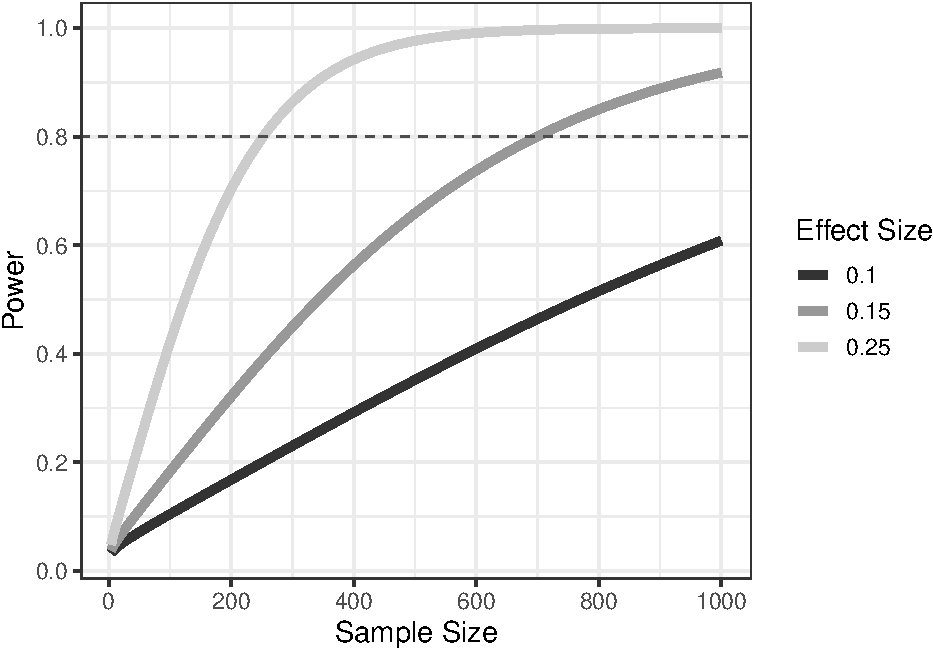
\includegraphics{power_simulation_files/figure-latex/vis-power-curve-1.pdf}

\hypertarget{two-sample-data-simulation-with-simglm}{%
\section{\texorpdfstring{Two sample Data simulation with \texttt{simglm}}{Two sample Data simulation with simglm}}\label{two-sample-data-simulation-with-simglm}}

The same two sample power analysis can be conducted by simulation with the \texttt{simglm} R package (LeBeau, 2019). This package simulates data based on general(-ized) linear (mixed) models. The two sample t-test shown above can be thought of as a linear model as well with a single indicator variable that specifies which group each data point belongs to.

\begin{Shaded}
\begin{Highlighting}[]
\NormalTok{simulation_arguments <-}\StringTok{ }\KeywordTok{list}\NormalTok{(}
  \DataTypeTok{formula =}\NormalTok{ y }\OperatorTok{~}\StringTok{ }\DecValTok{1} \OperatorTok{+}\StringTok{ }\NormalTok{sex,}
  \DataTypeTok{fixed =} \KeywordTok{list}\NormalTok{(}\DataTypeTok{sex =} \KeywordTok{list}\NormalTok{(}\DataTypeTok{var_type =} \StringTok{'factor'}\NormalTok{, }
                            \DataTypeTok{levels =} \KeywordTok{c}\NormalTok{(}\StringTok{'male'}\NormalTok{, }\StringTok{'female'}\NormalTok{))),}
  \DataTypeTok{sample_size =} \DecValTok{20}\NormalTok{,}
  \DataTypeTok{error =} \KeywordTok{list}\NormalTok{(}\DataTypeTok{variance =} \DecValTok{1}\NormalTok{),}
  \DataTypeTok{reg_weights =} \KeywordTok{c}\NormalTok{(}\DecValTok{0}\NormalTok{, }\FloatTok{.15}\NormalTok{)}
\NormalTok{)}

\KeywordTok{simulate_fixed}\NormalTok{(}\DataTypeTok{data =} \OtherTok{NULL}\NormalTok{, simulation_arguments) }\OperatorTok
\StringTok{  }\KeywordTok{simulate_error}\NormalTok{(simulation_arguments) }\OperatorTok
\StringTok{  }\KeywordTok{generate_response}\NormalTok{(simulation_arguments)}
\end{Highlighting}
\end{Shaded}

\begin{verbatim}
##    X.Intercept. sex   sex1 level1_id      error fixed_outcome
## 1             1   1   male         1  2.2866454          0.15
## 2             1   1   male         2 -1.3888607          0.15
## 3             1   0 female         3 -0.2787888          0.00
## 4             1   0 female         4 -0.1333213          0.00
## 5             1   0 female         5  0.6359504          0.00
## 6             1   0 female         6 -0.2842529          0.00
## 7             1   1   male         7 -2.6564554          0.15
## 8             1   0 female         8 -2.4404669          0.00
## 9             1   1   male         9  1.3201133          0.15
## 10            1   0 female        10 -0.3066386          0.00
## 11            1   1   male        11 -1.7813084          0.15
## 12            1   0 female        12 -0.1719174          0.00
## 13            1   1   male        13  1.2146747          0.15
## 14            1   1   male        14  1.8951935          0.15
## 15            1   0 female        15 -0.4304691          0.00
## 16            1   0 female        16 -0.2572694          0.00
## 17            1   0 female        17 -1.7631631          0.00
## 18            1   0 female        18  0.4600974          0.00
## 19            1   1   male        19 -0.6399949          0.15
## 20            1   1   male        20  0.4554501          0.15
##    random_effects          y
## 1               0  2.4366454
## 2               0 -1.2388607
## 3               0 -0.2787888
## 4               0 -0.1333213
## 5               0  0.6359504
## 6               0 -0.2842529
## 7               0 -2.5064554
## 8               0 -2.4404669
## 9               0  1.4701133
## 10              0 -0.3066386
## 11              0 -1.6313084
## 12              0 -0.1719174
## 13              0  1.3646747
## 14              0  2.0451935
## 15              0 -0.4304691
## 16              0 -0.2572694
## 17              0 -1.7631631
## 18              0  0.4600974
## 19              0 -0.4899949
## 20              0  0.6054501
\end{verbatim}

\hypertarget{using-simglm-to-generate-power}{%
\subsection{\texorpdfstring{Using \texttt{simglm} to generate power}{Using simglm to generate power}}\label{using-simglm-to-generate-power}}

\begin{Shaded}
\begin{Highlighting}[]
\KeywordTok{plan}\NormalTok{(multiprocess)}

\NormalTok{simulation_arguments <-}\StringTok{ }\KeywordTok{list}\NormalTok{(}
  \DataTypeTok{formula =}\NormalTok{ y }\OperatorTok{~}\StringTok{ }\DecValTok{1} \OperatorTok{+}\StringTok{ }\NormalTok{sex,}
  \DataTypeTok{fixed =} \KeywordTok{list}\NormalTok{(}\DataTypeTok{sex =} \KeywordTok{list}\NormalTok{(}\DataTypeTok{var_type =} \StringTok{'factor'}\NormalTok{, }
                            \DataTypeTok{levels =} \KeywordTok{c}\NormalTok{(}\StringTok{'male'}\NormalTok{, }\StringTok{'female'}\NormalTok{))),}
  \DataTypeTok{sample_size =} \DecValTok{20}\NormalTok{,}
  \DataTypeTok{error =} \KeywordTok{list}\NormalTok{(}\DataTypeTok{variance =} \DecValTok{1}\NormalTok{),}
  \DataTypeTok{reg_weights =} \KeywordTok{c}\NormalTok{(}\DecValTok{0}\NormalTok{, }\FloatTok{.15}\NormalTok{),}
  \DataTypeTok{replications =} \DecValTok{1000}\NormalTok{,}
  \DataTypeTok{model_fit =} \KeywordTok{list}\NormalTok{(}\DataTypeTok{formula =}\NormalTok{ y }\OperatorTok{~}\StringTok{ }\DecValTok{1} \OperatorTok{+}\StringTok{ }\NormalTok{sex, }
                   \DataTypeTok{model_function =} \StringTok{'lm'}\NormalTok{),}
  \DataTypeTok{extract_coefficients =} \OtherTok{TRUE}
\NormalTok{)}

\NormalTok{replicate_sim <-}\StringTok{ }\KeywordTok{replicate_simulation}\NormalTok{(simulation_arguments)}
\end{Highlighting}
\end{Shaded}

\begin{Shaded}
\begin{Highlighting}[]
\NormalTok{replicate_sim }\OperatorTok
\StringTok{  }\KeywordTok{compute_statistics}\NormalTok{(simulation_arguments, }\DataTypeTok{power =} \OtherTok{TRUE}\NormalTok{,}
                     \DataTypeTok{type_1_error =} \OtherTok{FALSE}\NormalTok{, }\DataTypeTok{precision =} \OtherTok{TRUE}\NormalTok{)}
\end{Highlighting}
\end{Shaded}

\begin{verbatim}
## # A tibble: 2 x 8
##   term  avg_estimate power avg_test_stat param_estimate_~ avg_standard_er~
##   <chr>        <dbl> <dbl>         <dbl>            <dbl>            <dbl>
## 1 (Int~       0.0114 0.082        0.0351            0.329            0.324
## 2 sex         0.132  0.077        0.302             0.461            0.457
## # ... with 2 more variables: precision_ratio <dbl>, replications <dbl>
\end{verbatim}

\begin{Shaded}
\begin{Highlighting}[]
\NormalTok{simulation_arguments <-}\StringTok{ }\KeywordTok{list}\NormalTok{(}
  \DataTypeTok{formula =}\NormalTok{ y }\OperatorTok{~}\StringTok{ }\DecValTok{1} \OperatorTok{+}\StringTok{ }\NormalTok{sex, }
  \DataTypeTok{fixed =} \KeywordTok{list}\NormalTok{(}\DataTypeTok{sex =} \KeywordTok{list}\NormalTok{(}\DataTypeTok{var_type =} \StringTok{'factor'}\NormalTok{, }
                            \DataTypeTok{levels =} \KeywordTok{c}\NormalTok{(}\StringTok{'male'}\NormalTok{, }\StringTok{'female'}\NormalTok{))),}
  \DataTypeTok{error =} \KeywordTok{list}\NormalTok{(}\DataTypeTok{variance =} \DecValTok{1}\NormalTok{),}
  \DataTypeTok{reg_weights =} \KeywordTok{c}\NormalTok{(}\DecValTok{0}\NormalTok{, }\FloatTok{.15}\NormalTok{),}
  \DataTypeTok{replications =} \DecValTok{1000}\NormalTok{,}
  \DataTypeTok{model_fit =} \KeywordTok{list}\NormalTok{(}\DataTypeTok{formula =}\NormalTok{ y }\OperatorTok{~}\StringTok{ }\DecValTok{1} \OperatorTok{+}\StringTok{ }\NormalTok{sex,}
                   \DataTypeTok{model_function =} \StringTok{'lm'}\NormalTok{),}
  \DataTypeTok{power =} \KeywordTok{list}\NormalTok{(}
    \DataTypeTok{dist =} \StringTok{'qnorm'}\NormalTok{,}
    \DataTypeTok{alpha =} \FloatTok{.05}
\NormalTok{  ),}
  \DataTypeTok{extract_coefficients =} \OtherTok{TRUE}\NormalTok{,}
  \DataTypeTok{vary_arguments =} \KeywordTok{list}\NormalTok{(}
    \DataTypeTok{sample_size =} \KeywordTok{seq}\NormalTok{(}\DecValTok{20}\NormalTok{, }\DecValTok{2000}\NormalTok{, }\DecValTok{20}\NormalTok{) }
\NormalTok{  )}
\NormalTok{)}

\NormalTok{model_results <-}\StringTok{ }\KeywordTok{replicate_simulation}\NormalTok{(simulation_arguments) }
\end{Highlighting}
\end{Shaded}

\begin{Shaded}
\begin{Highlighting}[]
\NormalTok{power_results <-}\StringTok{ }\NormalTok{model_results }\OperatorTok
\StringTok{  }\KeywordTok{compute_statistics}\NormalTok{(simulation_arguments, }\DataTypeTok{power =} \OtherTok{TRUE}\NormalTok{,}
                     \DataTypeTok{type_1_error =} \OtherTok{FALSE}\NormalTok{, }\DataTypeTok{precision =} \OtherTok{TRUE}\NormalTok{)}
\end{Highlighting}
\end{Shaded}

\begin{Shaded}
\begin{Highlighting}[]
\NormalTok{power_results <-}\StringTok{ }\NormalTok{power_results }\OperatorTok
\StringTok{  }\KeywordTok{ungroup}\NormalTok{() }\OperatorTok
\StringTok{  }\KeywordTok{mutate}\NormalTok{(}\DataTypeTok{sample_size =} \KeywordTok{as.numeric}\NormalTok{(}\KeywordTok{as.character}\NormalTok{(sample_size))) }\OperatorTok
\StringTok{  }\KeywordTok{arrange}\NormalTok{(sample_size) }\OperatorTok
\StringTok{  }\KeywordTok{filter}\NormalTok{(term }\OperatorTok{==}\StringTok{ 'sex'}\NormalTok{)}
\KeywordTok{head}\NormalTok{(power_results, }\DataTypeTok{n =} \DecValTok{10}\NormalTok{)}
\end{Highlighting}
\end{Shaded}

\begin{verbatim}
## # A tibble: 10 x 9
##    sample_size term  avg_estimate power avg_test_stat param_estimate_~
##          <dbl> <chr>        <dbl> <dbl>         <dbl>            <dbl>
##  1          20 sex          0.158 0.08          0.350            0.449
##  2          40 sex          0.168 0.093         0.542            0.323
##  3          60 sex          0.153 0.083         0.595            0.260
##  4          80 sex          0.146 0.085         0.652            0.217
##  5         100 sex          0.151 0.132         0.759            0.204
##  6         120 sex          0.141 0.126         0.772            0.187
##  7         140 sex          0.144 0.135         0.862            0.166
##  8         160 sex          0.148 0.153         0.939            0.152
##  9         180 sex          0.153 0.18          1.03             0.146
## 10         200 sex          0.154 0.198         1.10             0.141
## # ... with 3 more variables: avg_standard_error <dbl>,
## #   precision_ratio <dbl>, replications <dbl>
\end{verbatim}

This result can then be explored visually to generate a power curve.

\begin{Shaded}
\begin{Highlighting}[]
\KeywordTok{ggplot}\NormalTok{(power_results, }\KeywordTok{aes}\NormalTok{(}\DataTypeTok{x =}\NormalTok{ sample_size, }\DataTypeTok{y =}\NormalTok{ power)) }\OperatorTok{+}\StringTok{ }
\StringTok{  }\KeywordTok{geom_point}\NormalTok{(}\DataTypeTok{size =} \FloatTok{1.5}\NormalTok{, }\DataTypeTok{color =} \StringTok{'gray40'}\NormalTok{) }\OperatorTok{+}\StringTok{ }
\StringTok{  }\KeywordTok{geom_hline}\NormalTok{(}\DataTypeTok{yintercept =} \FloatTok{0.8}\NormalTok{, }\DataTypeTok{linetype =} \DecValTok{2}\NormalTok{, }\DataTypeTok{color =} \StringTok{'gray30'}\NormalTok{) }\OperatorTok{+}\StringTok{ }
\StringTok{  }\KeywordTok{geom_smooth}\NormalTok{(}\DataTypeTok{linetype =} \DecValTok{1}\NormalTok{, }\DataTypeTok{size =} \DecValTok{1}\NormalTok{, }\DataTypeTok{se =} \OtherTok{FALSE}\NormalTok{) }\OperatorTok{+}
\StringTok{  }\KeywordTok{geom_vline}\NormalTok{(}\DataTypeTok{xintercept =} \DecValTok{1488}\NormalTok{, }\DataTypeTok{linetype =} \DecValTok{2}\NormalTok{, }\DataTypeTok{color =} \StringTok{'gray30'}\NormalTok{) }\OperatorTok{+}
\StringTok{  }\KeywordTok{scale_x_continuous}\NormalTok{(}\StringTok{"Sample Size"}\NormalTok{, }\DataTypeTok{breaks =} \KeywordTok{seq}\NormalTok{(}\DecValTok{0}\NormalTok{, }\DecValTok{2000}\NormalTok{, }\DecValTok{200}\NormalTok{)) }\OperatorTok{+}\StringTok{ }
\StringTok{  }\KeywordTok{scale_y_continuous}\NormalTok{(}\StringTok{"Power"}\NormalTok{, }\DataTypeTok{breaks =} \KeywordTok{seq}\NormalTok{(}\DecValTok{0}\NormalTok{, }\DecValTok{1}\NormalTok{, }\FloatTok{.2}\NormalTok{)) }\OperatorTok{+}
\StringTok{  }\KeywordTok{theme_bw}\NormalTok{(}\DataTypeTok{base_size =} \DecValTok{14}\NormalTok{)}
\end{Highlighting}
\end{Shaded}

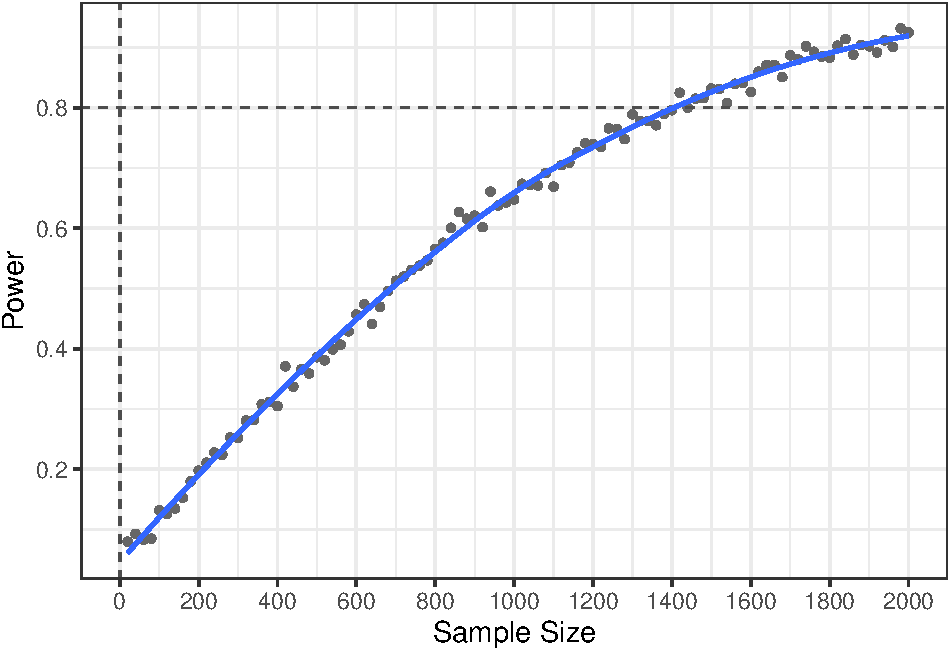
\includegraphics{power_simulation_files/figure-latex/simglm-power-curve-1.pdf}

\hypertarget{visualizing-estimates-and-p-values}{%
\subsection{Visualizing estimates and p-values}\label{visualizing-estimates-and-p-values}}

Exploring the estimates and the p-values can be informative over and above the power graphics shown above. The model results are stored in the object, \texttt{model\_results} shown above as a list for each replicated condition. This means that for each sample size, there are 1000 estimates for the group effect and the associated p-values based on these.

\begin{Shaded}
\begin{Highlighting}[]
\NormalTok{model_results_df <-}\StringTok{ }\KeywordTok{bind_rows}\NormalTok{(model_results) }\OperatorTok
\StringTok{  }\KeywordTok{filter}\NormalTok{(term }\OperatorTok{==}\StringTok{ 'sex'}\NormalTok{) }\OperatorTok
\StringTok{  }\KeywordTok{mutate}\NormalTok{(}\DataTypeTok{sample_size =} \KeywordTok{as.numeric}\NormalTok{(}\KeywordTok{as.character}\NormalTok{(sample_size)))}

\KeywordTok{ggplot}\NormalTok{(model_results_df, }\KeywordTok{aes}\NormalTok{(}\DataTypeTok{x =}\NormalTok{ sample_size, }\DataTypeTok{y =}\NormalTok{ estimate)) }\OperatorTok{+}\StringTok{ }
\StringTok{  }\KeywordTok{geom_boxplot}\NormalTok{(}\KeywordTok{aes}\NormalTok{(}\DataTypeTok{group =}\NormalTok{ sample_size), }\DataTypeTok{outlier.alpha =} \FloatTok{0.01}\NormalTok{) }\OperatorTok{+}
\StringTok{  }\KeywordTok{scale_x_continuous}\NormalTok{(}\StringTok{"Sample Size"}\NormalTok{, }\DataTypeTok{breaks =} \KeywordTok{seq}\NormalTok{(}\DecValTok{0}\NormalTok{, }\DecValTok{2000}\NormalTok{, }\DecValTok{200}\NormalTok{)) }\OperatorTok{+}
\StringTok{  }\KeywordTok{theme_bw}\NormalTok{(}\DataTypeTok{base_size =} \DecValTok{14}\NormalTok{) }\OperatorTok{+}
\StringTok{  }\KeywordTok{geom_hline}\NormalTok{(}\DataTypeTok{yintercept =} \FloatTok{.15}\NormalTok{, }\DataTypeTok{linetype =} \DecValTok{2}\NormalTok{, }\DataTypeTok{size =} \DecValTok{2}\NormalTok{, }\DataTypeTok{color =} \StringTok{'gray20'}\NormalTok{) }\OperatorTok{+}
\StringTok{  }\KeywordTok{coord_flip}\NormalTok{()}
\end{Highlighting}
\end{Shaded}

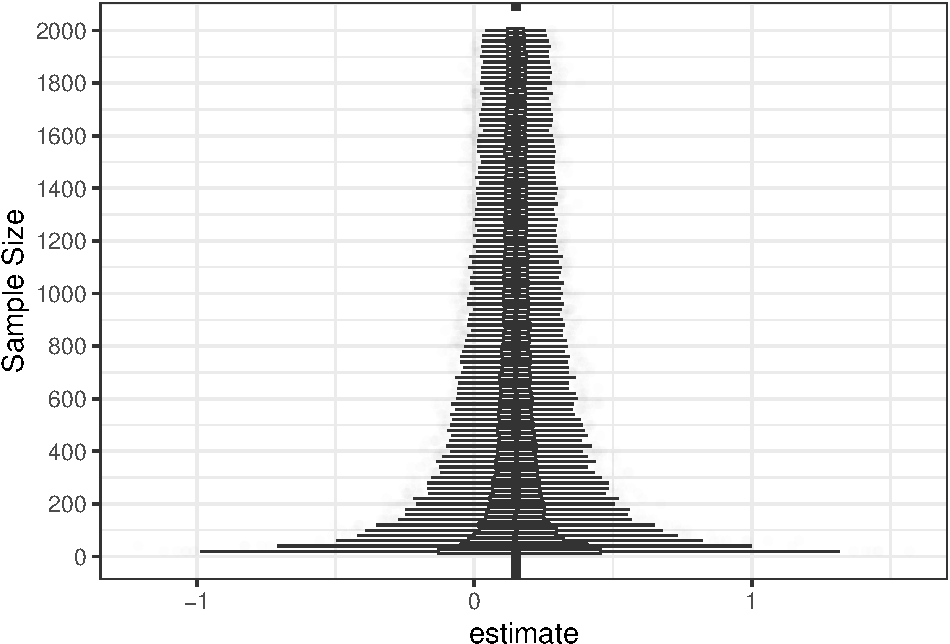
\includegraphics{power_simulation_files/figure-latex/estimate-figure-1.pdf}

\begin{Shaded}
\begin{Highlighting}[]
\KeywordTok{ggplot}\NormalTok{(model_results_df, }\KeywordTok{aes}\NormalTok{(}\DataTypeTok{x =}\NormalTok{ sample_size, }\DataTypeTok{y =}\NormalTok{ p.value)) }\OperatorTok{+}\StringTok{ }
\StringTok{  }\KeywordTok{geom_boxplot}\NormalTok{(}\KeywordTok{aes}\NormalTok{(}\DataTypeTok{group =}\NormalTok{ sample_size), }\DataTypeTok{outlier.alpha =} \FloatTok{0.01}\NormalTok{) }\OperatorTok{+}
\StringTok{  }\KeywordTok{scale_x_continuous}\NormalTok{(}\StringTok{"Sample Size"}\NormalTok{, }\DataTypeTok{breaks =} \KeywordTok{seq}\NormalTok{(}\DecValTok{0}\NormalTok{, }\DecValTok{2000}\NormalTok{, }\DecValTok{200}\NormalTok{)) }\OperatorTok{+}
\StringTok{  }\KeywordTok{theme_bw}\NormalTok{(}\DataTypeTok{base_size =} \DecValTok{14}\NormalTok{) }\OperatorTok{+}
\StringTok{  }\KeywordTok{geom_hline}\NormalTok{(}\DataTypeTok{yintercept =} \FloatTok{.05}\NormalTok{, }\DataTypeTok{linetype =} \DecValTok{2}\NormalTok{, }\DataTypeTok{size =} \DecValTok{2}\NormalTok{, }\DataTypeTok{color =} \StringTok{'gray20'}\NormalTok{) }\OperatorTok{+}
\StringTok{  }\KeywordTok{coord_flip}\NormalTok{()}
\end{Highlighting}
\end{Shaded}

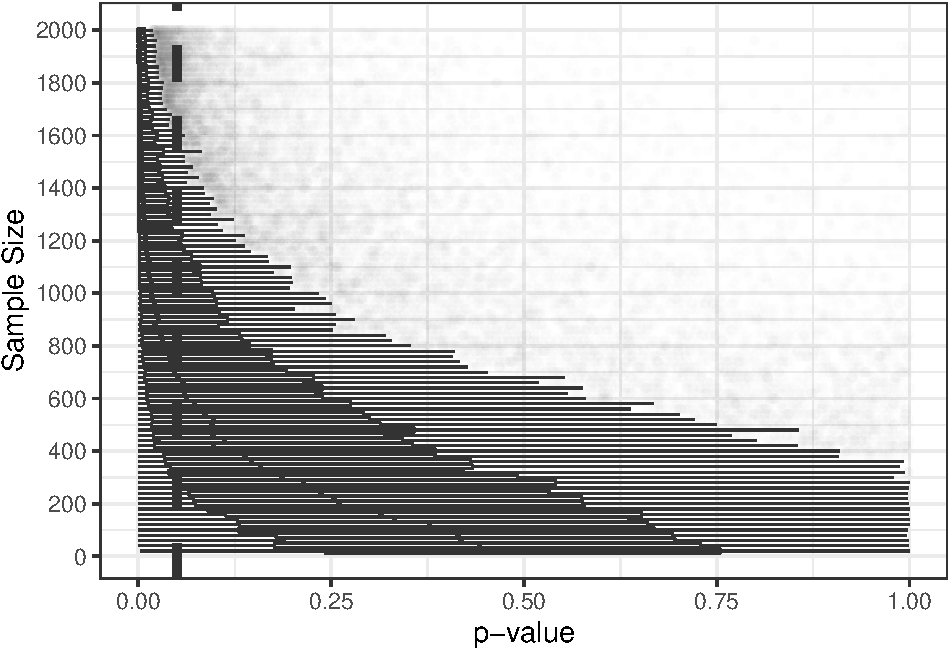
\includegraphics{power_simulation_files/figure-latex/p-value-figure-1.pdf}

\hypertarget{add-heterogeneity}{%
\subsection{Add Heterogeneity}\label{add-heterogeneity}}

Heterogeneity is a common phenomenon that can impact power and can occur when there are population variance differences across the two groups. In the above example, this would mean that there would be variance differences across males and females, perhaps males are more variable in the outcome. The \texttt{pwr.t.test()} function from before does not assume heterogeneity, however this is possible to incorporate when doing power from a simulation framework. Adding these conditions can help to mimic real world conditions and also maybe provide a better estimate of power.

\begin{Shaded}
\begin{Highlighting}[]
\NormalTok{simulation_arguments <-}\StringTok{ }\KeywordTok{list}\NormalTok{(}
  \DataTypeTok{formula =}\NormalTok{ y }\OperatorTok{~}\StringTok{ }\DecValTok{1} \OperatorTok{+}\StringTok{ }\NormalTok{group,}
  \DataTypeTok{fixed =} \KeywordTok{list}\NormalTok{(}\DataTypeTok{group =} \KeywordTok{list}\NormalTok{(}\DataTypeTok{var_type =} \StringTok{'factor'}\NormalTok{, }
                            \DataTypeTok{levels =} \KeywordTok{c}\NormalTok{(}\StringTok{'male'}\NormalTok{, }\StringTok{'female'}\NormalTok{))),}
  \DataTypeTok{error =} \KeywordTok{list}\NormalTok{(}\DataTypeTok{variance =} \DecValTok{1}\NormalTok{),}
  \DataTypeTok{heterogeneity =} \KeywordTok{list}\NormalTok{(}\DataTypeTok{variable =} \StringTok{'group'}\NormalTok{,}
                       \DataTypeTok{variance =} \KeywordTok{c}\NormalTok{(}\DecValTok{1}\NormalTok{, }\DecValTok{8}\NormalTok{)),}
  \DataTypeTok{reg_weights =} \KeywordTok{c}\NormalTok{(}\DecValTok{0}\NormalTok{, }\FloatTok{.15}\NormalTok{),}
  \DataTypeTok{replications =} \DecValTok{1000}\NormalTok{,}
  \DataTypeTok{model_fit =} \KeywordTok{list}\NormalTok{(}\DataTypeTok{formula =}\NormalTok{ y }\OperatorTok{~}\StringTok{ }\DecValTok{1} \OperatorTok{+}\StringTok{ }\NormalTok{group, }
                   \DataTypeTok{model_function =} \StringTok{'lm'}\NormalTok{),}
  \DataTypeTok{power =} \KeywordTok{list}\NormalTok{(}
    \DataTypeTok{dist =} \StringTok{'qnorm'}\NormalTok{,}
    \DataTypeTok{alpha =} \FloatTok{.05}
\NormalTok{  ),}
  \DataTypeTok{extract_coefficients =} \OtherTok{TRUE}\NormalTok{,}
  \DataTypeTok{vary_arguments =} \KeywordTok{list}\NormalTok{(}
    \DataTypeTok{sample_size =} \KeywordTok{seq}\NormalTok{(}\DecValTok{20}\NormalTok{, }\DecValTok{2000}\NormalTok{, }\DecValTok{20}\NormalTok{) }
\NormalTok{  )}
\NormalTok{)}

\NormalTok{model_results_h <-}\StringTok{ }\KeywordTok{replicate_simulation}\NormalTok{(simulation_arguments)}
\end{Highlighting}
\end{Shaded}

\begin{Shaded}
\begin{Highlighting}[]
\NormalTok{power_results_h <-}\StringTok{ }\NormalTok{model_results_h }\OperatorTok
\StringTok{  }\KeywordTok{compute_statistics}\NormalTok{(simulation_arguments, }\DataTypeTok{power =} \OtherTok{TRUE}\NormalTok{,}
                     \DataTypeTok{type_1_error =} \OtherTok{FALSE}\NormalTok{, }\DataTypeTok{precision =} \OtherTok{TRUE}\NormalTok{) }\OperatorTok
\StringTok{  }\KeywordTok{ungroup}\NormalTok{() }\OperatorTok
\StringTok{  }\KeywordTok{mutate}\NormalTok{(}\DataTypeTok{sample_size =} \KeywordTok{as.numeric}\NormalTok{(}\KeywordTok{as.character}\NormalTok{(sample_size)),}
         \DataTypeTok{heterogeneity =} \OtherTok{TRUE}\NormalTok{) }\OperatorTok
\StringTok{  }\KeywordTok{arrange}\NormalTok{(sample_size) }\OperatorTok
\StringTok{  }\KeywordTok{filter}\NormalTok{(term }\OperatorTok{==}\StringTok{ 'group'}\NormalTok{)}

\NormalTok{power_results <-}\StringTok{ }\NormalTok{power_results }\OperatorTok
\StringTok{  }\KeywordTok{mutate}\NormalTok{(}\DataTypeTok{heterogeneity =} \OtherTok{FALSE}\NormalTok{)}

\NormalTok{power_results_combined <-}\StringTok{ }\KeywordTok{bind_rows}\NormalTok{(power_results, }
\NormalTok{                                    power_results_h)}
\end{Highlighting}
\end{Shaded}

\begin{Shaded}
\begin{Highlighting}[]
\KeywordTok{ggplot}\NormalTok{(power_results_combined, }\KeywordTok{aes}\NormalTok{(}\DataTypeTok{x =}\NormalTok{ sample_size, }\DataTypeTok{y =}\NormalTok{ power, }
                          \DataTypeTok{group =}\NormalTok{ heterogeneity)) }\OperatorTok{+}\StringTok{ }
\StringTok{  }\KeywordTok{geom_point}\NormalTok{(}\KeywordTok{aes}\NormalTok{(}\DataTypeTok{shape =}\NormalTok{ heterogeneity), }\DataTypeTok{size =} \FloatTok{1.5}\NormalTok{, }\DataTypeTok{color =} \StringTok{'gray40'}\NormalTok{) }\OperatorTok{+}\StringTok{ }
\StringTok{  }\KeywordTok{geom_hline}\NormalTok{(}\DataTypeTok{yintercept =} \FloatTok{0.8}\NormalTok{, }\DataTypeTok{linetype =} \DecValTok{2}\NormalTok{, }\DataTypeTok{color =} \StringTok{'gray30'}\NormalTok{) }\OperatorTok{+}\StringTok{ }
\StringTok{  }\KeywordTok{geom_smooth}\NormalTok{(}\KeywordTok{aes}\NormalTok{(}\DataTypeTok{linetype =}\NormalTok{ heterogeneity), }\DataTypeTok{size =} \DecValTok{1}\NormalTok{, }\DataTypeTok{se =} \OtherTok{FALSE}\NormalTok{) }\OperatorTok{+}
\StringTok{  }\CommentTok{#geom_vline(xintercept = 1488, linetype = 2, color = 'gray30') +}
\StringTok{  }\KeywordTok{scale_x_continuous}\NormalTok{(}\StringTok{"Sample Size"}\NormalTok{, }\DataTypeTok{breaks =} \KeywordTok{seq}\NormalTok{(}\DecValTok{0}\NormalTok{, }\DecValTok{2000}\NormalTok{, }\DecValTok{200}\NormalTok{)) }\OperatorTok{+}\StringTok{ }
\StringTok{  }\KeywordTok{scale_y_continuous}\NormalTok{(}\StringTok{"Power"}\NormalTok{, }\DataTypeTok{breaks =} \KeywordTok{seq}\NormalTok{(}\DecValTok{0}\NormalTok{, }\DecValTok{1}\NormalTok{, }\FloatTok{.2}\NormalTok{)) }\OperatorTok{+}
\StringTok{  }\KeywordTok{theme_bw}\NormalTok{(}\DataTypeTok{base_size =} \DecValTok{14}\NormalTok{)}
\end{Highlighting}
\end{Shaded}

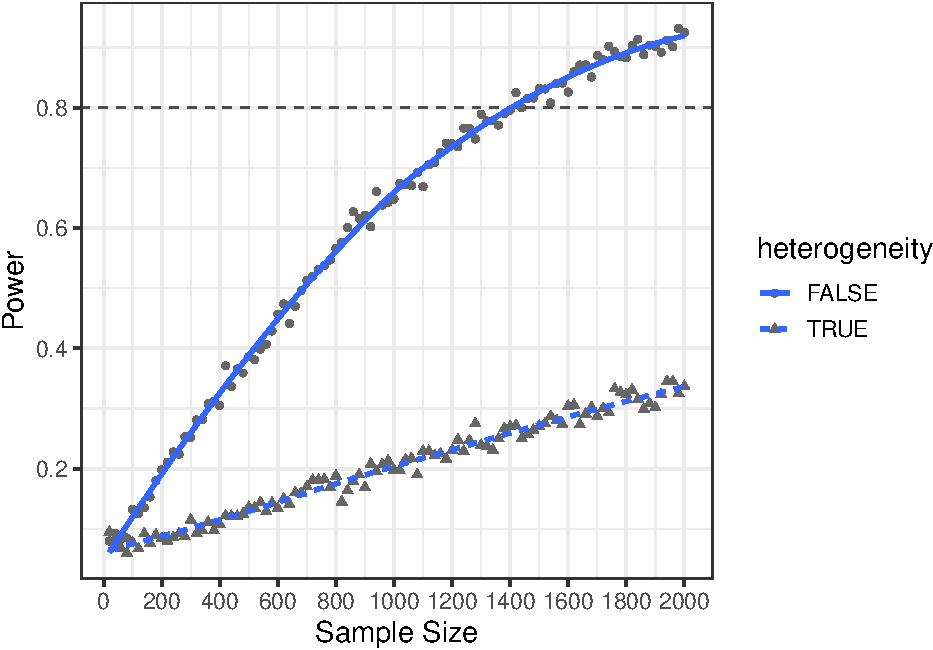
\includegraphics{power_simulation_files/figure-latex/simglm-power-curve-h-1.pdf}

\hypertarget{repeated-measures-example}{%
\section{Repeated Measures Example}\label{repeated-measures-example}}

For more complicated designs, closed form solutions are not always possible as ways to estimate statistical power or they make strong assumptions on the data that may not be reasonable given the data that are to be collected. The data simulation for the repeated measures portion adds a hierarchical data structure in which repeated measures are nested within individuals. These type of data add a correlation structure that needs to be modeled appropriately for valid inferences. Modern models to handle this dependency include the linear mixed model (LMM), sometimes known as the hierarchical linear model (HLM) or multilevel model.

This framework is an extension of the linear model considered above in the two group model. The extension includes the addition of random effects which represent subject specific deviations from the average trejectories. These random effects are what account for the dependency due to repeated measurements and nested data structure. In addition to the addition of random effects, two sample sizes need to be given, one representing the number of measurement occasions for each individual and another representing how individuals to generate. Therefore, in the balanced case (i.e.~same number of measurement occasions for each individual), the total sample size (i.e.~number of rows in the data) will be the number of measurement occasions times the number of individuals. This is a good initial check to ensure that the number of records are correct.

\begin{Shaded}
\begin{Highlighting}[]
\NormalTok{sim_arguments <-}\StringTok{ }\KeywordTok{list}\NormalTok{(}
  \DataTypeTok{formula =}\NormalTok{ y }\OperatorTok{~}\StringTok{ }\DecValTok{1} \OperatorTok{+}\StringTok{ }\NormalTok{time }\OperatorTok{+}\StringTok{ }\NormalTok{sex }\OperatorTok{+}\StringTok{ }\NormalTok{time}\OperatorTok{:}\NormalTok{sex }\OperatorTok{+}\StringTok{ }\NormalTok{(}\DecValTok{1} \OperatorTok{+}\StringTok{ }\NormalTok{time }\OperatorTok{|}\StringTok{ }\NormalTok{individual),}
  \DataTypeTok{reg_weights =} \KeywordTok{c}\NormalTok{(}\DecValTok{4}\NormalTok{, }\FloatTok{0.4}\NormalTok{, }\FloatTok{0.3}\NormalTok{, }\FloatTok{0.20}\NormalTok{),}
  \DataTypeTok{error =} \KeywordTok{list}\NormalTok{(}\DataTypeTok{variance =} \DecValTok{1}\NormalTok{),}
  \DataTypeTok{fixed =} \KeywordTok{list}\NormalTok{(}\DataTypeTok{time =} \KeywordTok{list}\NormalTok{(}\DataTypeTok{var_type =} \StringTok{'time'}\NormalTok{),}
               \DataTypeTok{sex =} \KeywordTok{list}\NormalTok{(}\DataTypeTok{var_type =} \StringTok{'factor'}\NormalTok{, }\DataTypeTok{levels =} \KeywordTok{c}\NormalTok{(}\StringTok{'male'}\NormalTok{, }\StringTok{'female'}\NormalTok{),}
                          \DataTypeTok{var_level =} \DecValTok{2}\NormalTok{)),}
  \DataTypeTok{randomeffect =} \KeywordTok{list}\NormalTok{(}\DataTypeTok{int_individual =} \KeywordTok{list}\NormalTok{(}\DataTypeTok{variance =} \DecValTok{1}\NormalTok{, }\DataTypeTok{var_level =} \DecValTok{2}\NormalTok{),}
                      \DataTypeTok{time_individual =} \KeywordTok{list}\NormalTok{(}\DataTypeTok{variance =} \FloatTok{0.5}\NormalTok{, }\DataTypeTok{var_level =} \DecValTok{2}\NormalTok{)),}
  \DataTypeTok{sample_size =} \KeywordTok{list}\NormalTok{(}\DataTypeTok{level1 =} \DecValTok{10}\NormalTok{, }\DataTypeTok{level2 =} \DecValTok{500}\NormalTok{)}
\NormalTok{)}

\NormalTok{longitudinal_data <-}\StringTok{ }\NormalTok{sim_arguments }\OperatorTok
\StringTok{  }\KeywordTok{simulate_fixed}\NormalTok{(}\DataTypeTok{data =} \OtherTok{NULL}\NormalTok{, .) }\OperatorTok
\StringTok{  }\KeywordTok{simulate_randomeffect}\NormalTok{(sim_arguments) }\OperatorTok
\StringTok{  }\KeywordTok{simulate_error}\NormalTok{(sim_arguments) }\OperatorTok
\StringTok{  }\KeywordTok{generate_response}\NormalTok{(sim_arguments)}
\end{Highlighting}
\end{Shaded}

\hypertarget{power-for-repeated-measures}{%
\subsection{Power for Repeated Measures}\label{power-for-repeated-measures}}

\begin{Shaded}
\begin{Highlighting}[]
\NormalTok{sim_arguments <-}\StringTok{ }\KeywordTok{list}\NormalTok{(}
  \DataTypeTok{formula =}\NormalTok{ y }\OperatorTok{~}\StringTok{ }\DecValTok{1} \OperatorTok{+}\StringTok{ }\NormalTok{time }\OperatorTok{+}\StringTok{ }\NormalTok{sex }\OperatorTok{+}\StringTok{ }\NormalTok{time}\OperatorTok{:}\NormalTok{sex }\OperatorTok{+}\StringTok{ }\NormalTok{(}\DecValTok{1} \OperatorTok{+}\StringTok{ }\NormalTok{time }\OperatorTok{|}\StringTok{ }\NormalTok{individual),}
  \DataTypeTok{reg_weights =} \KeywordTok{c}\NormalTok{(}\DecValTok{4}\NormalTok{, }\FloatTok{0.4}\NormalTok{, }\FloatTok{0.3}\NormalTok{, }\FloatTok{0.20}\NormalTok{),}
  \DataTypeTok{error =} \KeywordTok{list}\NormalTok{(}\DataTypeTok{variance =} \DecValTok{1}\NormalTok{),}
  \DataTypeTok{fixed =} \KeywordTok{list}\NormalTok{(}\DataTypeTok{time =} \KeywordTok{list}\NormalTok{(}\DataTypeTok{var_type =} \StringTok{'time'}\NormalTok{),}
               \DataTypeTok{sex =} \KeywordTok{list}\NormalTok{(}\DataTypeTok{var_type =} \StringTok{'factor'}\NormalTok{, }\DataTypeTok{levels =} \KeywordTok{c}\NormalTok{(}\StringTok{'male'}\NormalTok{, }\StringTok{'female'}\NormalTok{),}
                          \DataTypeTok{var_level =} \DecValTok{2}\NormalTok{)),}
  \DataTypeTok{randomeffect =} \KeywordTok{list}\NormalTok{(}\DataTypeTok{int_individual =} \KeywordTok{list}\NormalTok{(}\DataTypeTok{variance =} \DecValTok{1}\NormalTok{, }\DataTypeTok{var_level =} \DecValTok{2}\NormalTok{),}
                      \DataTypeTok{time_individual =} \KeywordTok{list}\NormalTok{(}\DataTypeTok{variance =} \FloatTok{0.5}\NormalTok{, }\DataTypeTok{var_level =} \DecValTok{2}\NormalTok{)),}
  \DataTypeTok{sample_size =} \KeywordTok{list}\NormalTok{(}\DataTypeTok{level1 =} \DecValTok{10}\NormalTok{, }\DataTypeTok{level2 =} \DecValTok{500}\NormalTok{),}
  \DataTypeTok{replications =} \DecValTok{1000}\NormalTok{,}
  \DataTypeTok{model_fit =} \KeywordTok{list}\NormalTok{(}\DataTypeTok{formula =}\NormalTok{ y }\OperatorTok{~}\StringTok{ }\DecValTok{1} \OperatorTok{+}\StringTok{ }\NormalTok{time }\OperatorTok{+}\StringTok{ }\NormalTok{sex }\OperatorTok{+}\StringTok{ }\NormalTok{time}\OperatorTok{:}\NormalTok{sex }\OperatorTok{+}\StringTok{ }
\StringTok{                     }\NormalTok{(}\DecValTok{1} \OperatorTok{+}\StringTok{ }\NormalTok{time }\OperatorTok{|}\StringTok{ }\NormalTok{individual), }
                   \DataTypeTok{model_function =} \StringTok{'lmer'}\NormalTok{),}
  \DataTypeTok{extract_coefficients =} \OtherTok{TRUE}
\NormalTok{)}

\NormalTok{long_models <-}\StringTok{ }\KeywordTok{replicate_simulation}\NormalTok{(sim_arguments)}
\end{Highlighting}
\end{Shaded}

\begin{Shaded}
\begin{Highlighting}[]
\NormalTok{long_models }\OperatorTok
\StringTok{  }\KeywordTok{compute_statistics}\NormalTok{(sim_arguments, }\DataTypeTok{power =} \OtherTok{TRUE}\NormalTok{,}
                     \DataTypeTok{type_1_error =} \OtherTok{FALSE}\NormalTok{, }\DataTypeTok{precision =} \OtherTok{TRUE}\NormalTok{)}
\end{Highlighting}
\end{Shaded}

\begin{verbatim}
## # A tibble: 4 x 8
##   term  avg_estimate power avg_test_stat param_estimate_~ avg_standard_er~
##   <fct>        <dbl> <dbl>         <dbl>            <dbl>            <dbl>
## 1 (Int~        4.00  1             54.6            0.0749           0.0734
## 2 sex          0.300 0.819          2.89           0.108            0.104 
## 3 time         0.403 1              8.94           0.0434           0.0452
## 4 time~        0.199 0.872          3.11           0.0613           0.0639
## # ... with 2 more variables: precision_ratio <dbl>, replications <dbl>
\end{verbatim}

\hypertarget{varying-simulation-conditions}{%
\subsubsection{Varying simulation conditions}\label{varying-simulation-conditions}}

\begin{Shaded}
\begin{Highlighting}[]
\NormalTok{sim_arguments <-}\StringTok{ }\KeywordTok{list}\NormalTok{(}
  \DataTypeTok{formula =}\NormalTok{ y }\OperatorTok{~}\StringTok{ }\DecValTok{1} \OperatorTok{+}\StringTok{ }\NormalTok{time }\OperatorTok{+}\StringTok{ }\NormalTok{sex }\OperatorTok{+}\StringTok{ }\NormalTok{time}\OperatorTok{:}\NormalTok{sex }\OperatorTok{+}\StringTok{ }\NormalTok{(}\DecValTok{1} \OperatorTok{+}\StringTok{ }\NormalTok{time }\OperatorTok{|}\StringTok{ }\NormalTok{individual),}
  \DataTypeTok{reg_weights =} \KeywordTok{c}\NormalTok{(}\DecValTok{4}\NormalTok{, }\FloatTok{0.4}\NormalTok{, }\FloatTok{0.3}\NormalTok{, }\FloatTok{0.20}\NormalTok{),}
  \DataTypeTok{error =} \KeywordTok{list}\NormalTok{(}\DataTypeTok{variance =} \DecValTok{1}\NormalTok{),}
  \DataTypeTok{fixed =} \KeywordTok{list}\NormalTok{(}\DataTypeTok{time =} \KeywordTok{list}\NormalTok{(}\DataTypeTok{var_type =} \StringTok{'time'}\NormalTok{),}
               \DataTypeTok{sex =} \KeywordTok{list}\NormalTok{(}\DataTypeTok{var_type =} \StringTok{'factor'}\NormalTok{, }\DataTypeTok{levels =} \KeywordTok{c}\NormalTok{(}\StringTok{'male'}\NormalTok{, }\StringTok{'female'}\NormalTok{),}
                          \DataTypeTok{var_level =} \DecValTok{2}\NormalTok{)),}
  \DataTypeTok{randomeffect =} \KeywordTok{list}\NormalTok{(}\DataTypeTok{int_individual =} \KeywordTok{list}\NormalTok{(}\DataTypeTok{variance =} \DecValTok{1}\NormalTok{, }\DataTypeTok{var_level =} \DecValTok{2}\NormalTok{),}
                      \DataTypeTok{time_individual =} \KeywordTok{list}\NormalTok{(}\DataTypeTok{variance =} \FloatTok{0.5}\NormalTok{, }\DataTypeTok{var_level =} \DecValTok{2}\NormalTok{)),}
  \DataTypeTok{replications =} \DecValTok{1000}\NormalTok{,}
  \DataTypeTok{model_fit =} \KeywordTok{list}\NormalTok{(}\DataTypeTok{formula =}\NormalTok{ y }\OperatorTok{~}\StringTok{ }\DecValTok{1} \OperatorTok{+}\StringTok{ }\NormalTok{time }\OperatorTok{+}\StringTok{ }\NormalTok{sex }\OperatorTok{+}\StringTok{ }\NormalTok{time}\OperatorTok{:}\NormalTok{sex }\OperatorTok{+}\StringTok{ }
\StringTok{                     }\NormalTok{(}\DecValTok{1} \OperatorTok{+}\StringTok{ }\NormalTok{time }\OperatorTok{|}\StringTok{ }\NormalTok{individual), }
                   \DataTypeTok{model_function =} \StringTok{'lmer'}\NormalTok{),}
  \DataTypeTok{extract_coefficients =} \OtherTok{TRUE}\NormalTok{,}
  \DataTypeTok{vary_arguments =} \KeywordTok{list}\NormalTok{(}
    \DataTypeTok{sample_size =} \KeywordTok{list}\NormalTok{(}\KeywordTok{list}\NormalTok{(}\DataTypeTok{level1 =} \DecValTok{5}\NormalTok{, }\DataTypeTok{level2 =} \DecValTok{50}\NormalTok{),}
                       \KeywordTok{list}\NormalTok{(}\DataTypeTok{level1 =} \DecValTok{5}\NormalTok{, }\DataTypeTok{level2 =} \DecValTok{150}\NormalTok{),}
                       \KeywordTok{list}\NormalTok{(}\DataTypeTok{level1 =} \DecValTok{5}\NormalTok{, }\DataTypeTok{level2 =} \DecValTok{250}\NormalTok{),}
                       \KeywordTok{list}\NormalTok{(}\DataTypeTok{level1 =} \DecValTok{8}\NormalTok{, }\DataTypeTok{level2 =} \DecValTok{50}\NormalTok{),}
                       \KeywordTok{list}\NormalTok{(}\DataTypeTok{level1 =} \DecValTok{8}\NormalTok{, }\DataTypeTok{level2 =} \DecValTok{150}\NormalTok{),}
                       \KeywordTok{list}\NormalTok{(}\DataTypeTok{level1 =} \DecValTok{8}\NormalTok{, }\DataTypeTok{level2 =} \DecValTok{250}\NormalTok{))}
\NormalTok{  )}
\NormalTok{)}

\NormalTok{long_model_nomiss <-}\StringTok{ }\KeywordTok{replicate_simulation}\NormalTok{(sim_arguments) }
\end{Highlighting}
\end{Shaded}

\begin{Shaded}
\begin{Highlighting}[]
\NormalTok{long_power_nomiss <-}\StringTok{ }\NormalTok{long_model_nomiss }\OperatorTok
\StringTok{  }\KeywordTok{compute_statistics}\NormalTok{(sim_arguments, }\DataTypeTok{power =} \OtherTok{TRUE}\NormalTok{,}
                     \DataTypeTok{type_1_error =} \OtherTok{FALSE}\NormalTok{, }\DataTypeTok{precision =} \OtherTok{TRUE}\NormalTok{)}
\end{Highlighting}
\end{Shaded}

\begin{Shaded}
\begin{Highlighting}[]
\NormalTok{sim_arguments <-}\StringTok{ }\KeywordTok{list}\NormalTok{(}
  \DataTypeTok{formula =}\NormalTok{ y }\OperatorTok{~}\StringTok{ }\DecValTok{1} \OperatorTok{+}\StringTok{ }\NormalTok{time }\OperatorTok{+}\StringTok{ }\NormalTok{sex }\OperatorTok{+}\StringTok{ }\NormalTok{time}\OperatorTok{:}\NormalTok{sex }\OperatorTok{+}\StringTok{ }\NormalTok{(}\DecValTok{1} \OperatorTok{+}\StringTok{ }\NormalTok{time }\OperatorTok{|}\StringTok{ }\NormalTok{individual),}
  \DataTypeTok{reg_weights =} \KeywordTok{c}\NormalTok{(}\DecValTok{4}\NormalTok{, }\FloatTok{0.4}\NormalTok{, }\FloatTok{0.3}\NormalTok{, }\FloatTok{0.20}\NormalTok{),}
  \DataTypeTok{error =} \KeywordTok{list}\NormalTok{(}\DataTypeTok{variance =} \DecValTok{1}\NormalTok{),}
  \DataTypeTok{fixed =} \KeywordTok{list}\NormalTok{(}\DataTypeTok{time =} \KeywordTok{list}\NormalTok{(}\DataTypeTok{var_type =} \StringTok{'time'}\NormalTok{),}
               \DataTypeTok{sex =} \KeywordTok{list}\NormalTok{(}\DataTypeTok{var_type =} \StringTok{'factor'}\NormalTok{, }\DataTypeTok{levels =} \KeywordTok{c}\NormalTok{(}\StringTok{'male'}\NormalTok{, }\StringTok{'female'}\NormalTok{),}
                          \DataTypeTok{var_level =} \DecValTok{2}\NormalTok{)),}
  \DataTypeTok{randomeffect =} \KeywordTok{list}\NormalTok{(}\DataTypeTok{int_individual =} \KeywordTok{list}\NormalTok{(}\DataTypeTok{variance =} \DecValTok{1}\NormalTok{, }\DataTypeTok{var_level =} \DecValTok{2}\NormalTok{),}
                      \DataTypeTok{time_individual =} \KeywordTok{list}\NormalTok{(}\DataTypeTok{variance =} \FloatTok{0.5}\NormalTok{, }\DataTypeTok{var_level =} \DecValTok{2}\NormalTok{)),}
  \DataTypeTok{replications =} \DecValTok{1000}\NormalTok{,}
  \DataTypeTok{model_fit =} \KeywordTok{list}\NormalTok{(}\DataTypeTok{formula =}\NormalTok{ y_miss }\OperatorTok{~}\StringTok{ }\DecValTok{1} \OperatorTok{+}\StringTok{ }\NormalTok{time }\OperatorTok{+}\StringTok{ }\NormalTok{sex }\OperatorTok{+}\StringTok{ }\NormalTok{time}\OperatorTok{:}\NormalTok{sex }\OperatorTok{+}\StringTok{ }
\StringTok{                     }\NormalTok{(}\DecValTok{1} \OperatorTok{+}\StringTok{ }\NormalTok{time }\OperatorTok{|}\StringTok{ }\NormalTok{individual), }
                   \DataTypeTok{model_function =} \StringTok{'lmer'}\NormalTok{),}
  \DataTypeTok{missing_data =} \KeywordTok{list}\NormalTok{(}\DataTypeTok{new_outcome =} \StringTok{'y_miss'}\NormalTok{, }\DataTypeTok{miss_prop =} \FloatTok{.20}\NormalTok{,}
                      \DataTypeTok{clust_var =} \StringTok{'individual'}\NormalTok{, }\DataTypeTok{type =} \StringTok{'dropout'}\NormalTok{),}
  \DataTypeTok{extract_coefficients =} \OtherTok{TRUE}\NormalTok{,}
  \DataTypeTok{vary_arguments =} \KeywordTok{list}\NormalTok{(}
    \DataTypeTok{sample_size =} \KeywordTok{list}\NormalTok{(}\KeywordTok{list}\NormalTok{(}\DataTypeTok{level1 =} \DecValTok{5}\NormalTok{, }\DataTypeTok{level2 =} \DecValTok{50}\NormalTok{),}
                       \KeywordTok{list}\NormalTok{(}\DataTypeTok{level1 =} \DecValTok{5}\NormalTok{, }\DataTypeTok{level2 =} \DecValTok{150}\NormalTok{),}
                       \KeywordTok{list}\NormalTok{(}\DataTypeTok{level1 =} \DecValTok{5}\NormalTok{, }\DataTypeTok{level2 =} \DecValTok{250}\NormalTok{),}
                       \KeywordTok{list}\NormalTok{(}\DataTypeTok{level1 =} \DecValTok{8}\NormalTok{, }\DataTypeTok{level2 =} \DecValTok{50}\NormalTok{),}
                       \KeywordTok{list}\NormalTok{(}\DataTypeTok{level1 =} \DecValTok{8}\NormalTok{, }\DataTypeTok{level2 =} \DecValTok{150}\NormalTok{),}
                       \KeywordTok{list}\NormalTok{(}\DataTypeTok{level1 =} \DecValTok{8}\NormalTok{, }\DataTypeTok{level2 =} \DecValTok{250}\NormalTok{))}
\NormalTok{  )}
\NormalTok{)}

\NormalTok{long_model_miss <-}\StringTok{ }\KeywordTok{replicate_simulation}\NormalTok{(sim_arguments) }
\end{Highlighting}
\end{Shaded}

\begin{Shaded}
\begin{Highlighting}[]
\NormalTok{long_power_miss <-}\StringTok{ }\NormalTok{long_model_miss }\OperatorTok
\StringTok{  }\KeywordTok{compute_statistics}\NormalTok{(sim_arguments, }\DataTypeTok{power =} \OtherTok{TRUE}\NormalTok{,}
                     \DataTypeTok{type_1_error =} \OtherTok{FALSE}\NormalTok{, }\DataTypeTok{precision =} \OtherTok{TRUE}\NormalTok{)}
\end{Highlighting}
\end{Shaded}

\begin{Shaded}
\begin{Highlighting}[]
\NormalTok{long_power_nomiss_h <-}\StringTok{ }\NormalTok{long_power_nomiss }\OperatorTok
\StringTok{  }\KeywordTok{ungroup}\NormalTok{() }\OperatorTok
\StringTok{  }\KeywordTok{mutate}\NormalTok{(}\DataTypeTok{sample_size =} \KeywordTok{gsub}\NormalTok{(}\StringTok{"^list}\CharTok{\textbackslash{}\textbackslash{}}\StringTok{(|}\CharTok{\textbackslash{}\textbackslash{}}\StringTok{)$"}\NormalTok{, }\StringTok{""}\NormalTok{, }\KeywordTok{as.character}\NormalTok{(sample_size)),}
         \DataTypeTok{missing =} \OtherTok{FALSE}\NormalTok{)}

\NormalTok{long_power_miss_h <-}\StringTok{ }\NormalTok{long_power_miss }\OperatorTok
\StringTok{  }\KeywordTok{ungroup}\NormalTok{() }\OperatorTok
\StringTok{  }\KeywordTok{mutate}\NormalTok{(}\DataTypeTok{sample_size =} \KeywordTok{gsub}\NormalTok{(}\StringTok{"^list}\CharTok{\textbackslash{}\textbackslash{}}\StringTok{(|}\CharTok{\textbackslash{}\textbackslash{}}\StringTok{)$"}\NormalTok{, }\StringTok{""}\NormalTok{, }\KeywordTok{as.character}\NormalTok{(sample_size)), }
         \DataTypeTok{missing =} \OtherTok{TRUE}\NormalTok{)}

\NormalTok{long_power_combined <-}\StringTok{ }\KeywordTok{bind_rows}\NormalTok{(long_power_nomiss_h, }
\NormalTok{                                    long_power_miss_h)}
\end{Highlighting}
\end{Shaded}

\begin{Shaded}
\begin{Highlighting}[]
\NormalTok{long_power_sex <-}\StringTok{ }\KeywordTok{filter}\NormalTok{(long_power_combined, term }\OperatorTok{==}\StringTok{ 'sex'}\NormalTok{)}

\KeywordTok{ggplot}\NormalTok{(long_power_sex, }\KeywordTok{aes}\NormalTok{(}\DataTypeTok{x =} \KeywordTok{reorder}\NormalTok{(sample_size, }\KeywordTok{desc}\NormalTok{(power)), }\DataTypeTok{y =}\NormalTok{ power, }
                          \DataTypeTok{group =}\NormalTok{ missing)) }\OperatorTok{+}\StringTok{ }
\StringTok{  }\KeywordTok{geom_point}\NormalTok{(}\KeywordTok{aes}\NormalTok{(}\DataTypeTok{shape =}\NormalTok{ missing), }\DataTypeTok{size =} \FloatTok{1.5}\NormalTok{, }\DataTypeTok{color =} \StringTok{'gray40'}\NormalTok{) }\OperatorTok{+}\StringTok{ }
\StringTok{  }\KeywordTok{geom_line}\NormalTok{(}\KeywordTok{aes}\NormalTok{(}\DataTypeTok{linetype =}\NormalTok{ missing), }\DataTypeTok{size =} \DecValTok{1}\NormalTok{) }\OperatorTok{+}
\StringTok{  }\KeywordTok{geom_hline}\NormalTok{(}\DataTypeTok{yintercept =} \FloatTok{0.8}\NormalTok{, }\DataTypeTok{linetype =} \DecValTok{2}\NormalTok{, }\DataTypeTok{color =} \StringTok{'gray30'}\NormalTok{) }\OperatorTok{+}\StringTok{ }
\StringTok{  }\CommentTok{#geom_smooth(aes(linetype = missing), size = 1, se = FALSE) +}
\StringTok{  }\CommentTok{#geom_vline(xintercept = 1488, linetype = 2, color = 'gray30') +}
\StringTok{  }\KeywordTok{xlab}\NormalTok{(}\StringTok{"Sample Size"}\NormalTok{) }\OperatorTok{+}\StringTok{ }
\StringTok{  }\KeywordTok{scale_y_continuous}\NormalTok{(}\StringTok{"Power"}\NormalTok{, }\DataTypeTok{breaks =} \KeywordTok{seq}\NormalTok{(}\DecValTok{0}\NormalTok{, }\DecValTok{1}\NormalTok{, }\FloatTok{.2}\NormalTok{), }\DataTypeTok{limits =} \KeywordTok{c}\NormalTok{(}\DecValTok{0}\NormalTok{, }\DecValTok{1}\NormalTok{)) }\OperatorTok{+}
\StringTok{  }\KeywordTok{theme_bw}\NormalTok{(}\DataTypeTok{base_size =} \DecValTok{14}\NormalTok{) }\OperatorTok{+}\StringTok{ }
\StringTok{  }\KeywordTok{coord_flip}\NormalTok{()}
\end{Highlighting}
\end{Shaded}

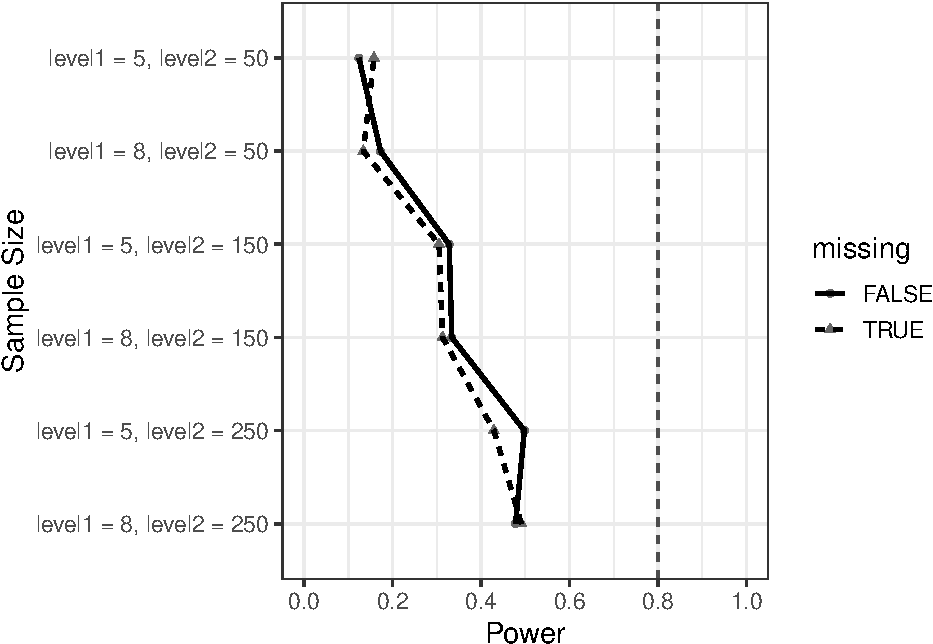
\includegraphics{power_simulation_files/figure-latex/long-power-curve-h-1.pdf}

\begin{Shaded}
\begin{Highlighting}[]
\NormalTok{long_power_timesex <-}\StringTok{ }\KeywordTok{filter}\NormalTok{(long_power_combined, term }\OperatorTok{==}\StringTok{ 'time:sex'}\NormalTok{)}

\KeywordTok{ggplot}\NormalTok{(long_power_timesex, }\KeywordTok{aes}\NormalTok{(}\DataTypeTok{x =} \KeywordTok{reorder}\NormalTok{(sample_size, }\KeywordTok{desc}\NormalTok{(power)), }\DataTypeTok{y =}\NormalTok{ power, }
                          \DataTypeTok{group =}\NormalTok{ missing)) }\OperatorTok{+}\StringTok{ }
\StringTok{  }\KeywordTok{geom_point}\NormalTok{(}\KeywordTok{aes}\NormalTok{(}\DataTypeTok{shape =}\NormalTok{ missing), }\DataTypeTok{size =} \FloatTok{1.5}\NormalTok{, }\DataTypeTok{color =} \StringTok{'gray40'}\NormalTok{) }\OperatorTok{+}\StringTok{ }
\StringTok{  }\KeywordTok{geom_line}\NormalTok{(}\KeywordTok{aes}\NormalTok{(}\DataTypeTok{linetype =}\NormalTok{ missing), }\DataTypeTok{size =} \DecValTok{1}\NormalTok{) }\OperatorTok{+}
\StringTok{  }\KeywordTok{geom_hline}\NormalTok{(}\DataTypeTok{yintercept =} \FloatTok{0.8}\NormalTok{, }\DataTypeTok{linetype =} \DecValTok{2}\NormalTok{, }\DataTypeTok{color =} \StringTok{'gray30'}\NormalTok{) }\OperatorTok{+}\StringTok{ }
\StringTok{  }\CommentTok{#geom_smooth(aes(linetype = missing), size = 1, se = FALSE) +}
\StringTok{  }\CommentTok{#geom_vline(xintercept = 1488, linetype = 2, color = 'gray30') +}
\StringTok{  }\KeywordTok{xlab}\NormalTok{(}\StringTok{"Sample Size"}\NormalTok{) }\OperatorTok{+}\StringTok{ }
\StringTok{  }\KeywordTok{scale_y_continuous}\NormalTok{(}\StringTok{"Power"}\NormalTok{, }\DataTypeTok{breaks =} \KeywordTok{seq}\NormalTok{(}\DecValTok{0}\NormalTok{, }\DecValTok{1}\NormalTok{, }\FloatTok{.2}\NormalTok{), }\DataTypeTok{limits =} \KeywordTok{c}\NormalTok{(}\DecValTok{0}\NormalTok{, }\DecValTok{1}\NormalTok{)) }\OperatorTok{+}
\StringTok{  }\KeywordTok{theme_bw}\NormalTok{(}\DataTypeTok{base_size =} \DecValTok{14}\NormalTok{) }\OperatorTok{+}\StringTok{ }
\StringTok{  }\KeywordTok{coord_flip}\NormalTok{()}
\end{Highlighting}
\end{Shaded}

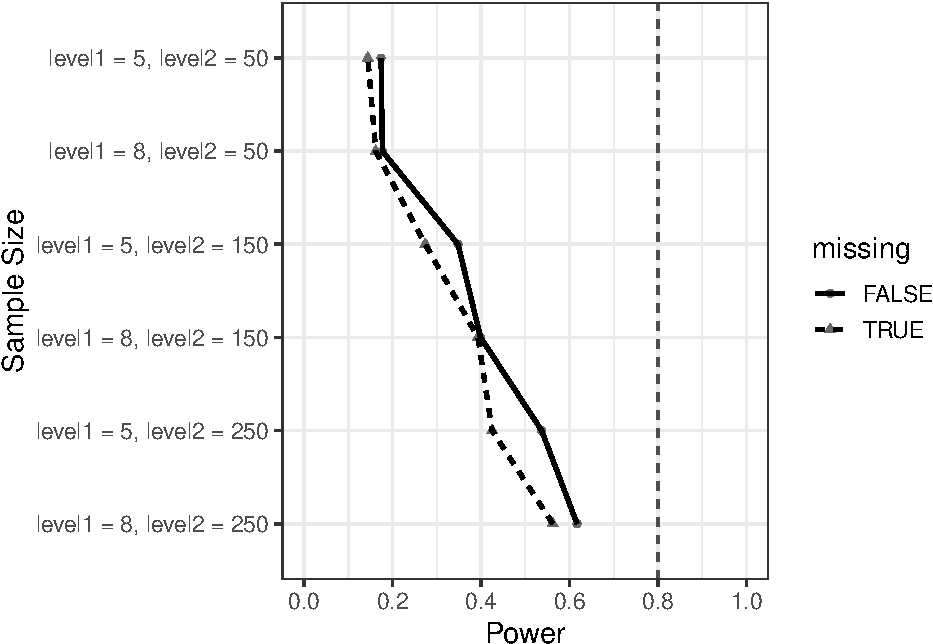
\includegraphics{power_simulation_files/figure-latex/long-power-curve-ts-1.pdf}

\hypertarget{summary}{%
\section{Summary}\label{summary}}

\newpage

\hypertarget{references}{%
\section{References}\label{references}}

\begingroup
\setlength{\parindent}{-0.5in}
\setlength{\leftskip}{0.5in}

\hypertarget{refs}{}
\leavevmode\hypertarget{ref-simglm}{}%
LeBeau, B. (2019). \emph{Simglm: Simulate models based on the generalized linear model}. Retrieved from \url{https://CRAN.R-project.org/package=simglm}

\endgroup


\end{document}
